\chapter{Разработка расчетной сетки и аппроксимация свойств местности на узлы сетки}

% План
% 1) Расчетная сетка в методе конечных элеменых элементов (какие бывают, почему именно такую выбрали)
% 2) Разработка расчетной сетки
% 3) Зависимость параметров уравнения от типа местности
% 4) Разработка кода апроксимации
% 5) Заключение

\section{Расчетная сетка в методе конечных элементов}

Для решения уравнения адвекции-диффузии, описанного в разделе \ref{diffusion_model}, в модели \ac{ascro} применяется 
метод конечных элементов. В этом методе область, в которой ищется решение уравнения, разбивается на конечное количество 
подоблостей. Каждая из этих подобластей называется элементами. В каждом элементе выбирается вид аппроксимирующей функции. 
Вне своего элемента аппроксимирующая функция равняется нулю. Значения функций в узлах элементов заранее неизвестны и 
являются решением задачи. Вначале ищутся коэффициенты аппроксимирующих функций из условия равенства соседних функций в 
узлах элементов. После этого, коэффициенты выражаются через значения функций в узлах элементов. Составляется система 
линейных алгебраических уравнений, количество уравнений в которой равно количеству неизвестных значений в узлах, в 
которых ищется решение системы. 

Расчетная сетка в модели \ac{ascro} имеет форму цилиндра и представляет собой участок местности вблизи \ac{aes}. 
Так как расчетная сетка имеет форму цилиндра, её элементы должны быть трехмерными.

Существует четыре основных типа трехмерных элементов: тетраэдры, гексаэдры, призмы и пирамиды (рисунок 
\ref{fig_finite_elements}). Самым распространенным элементом при построении расчетных сеток являются тетраэдры. 

\begin{figure}[ht]
\centering
	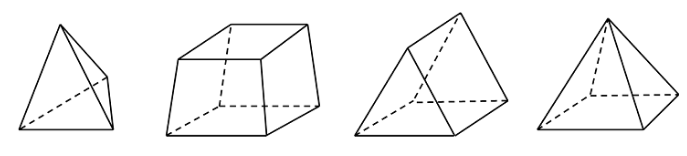
\includegraphics[width=16cm]{finite_elements}
	\captionsetup{justification=centering}
    \caption{Основные типы трехмерных элементов расчетной сетки.}
    \label{fig_finite_elements}
\end{figure}

Тетраэдрический элемент является простейшим элементом и позволяет построить расчетную сетку практически для любого 
трёхмерного тела. В модели \ac{ascro} для решения уравнения адвекции-диффузии методом конечных элементов используется 
расчетная сетка с тетраэдрическими элементами.

\section{Создание расчетной сетки}

Построение расчетной сетки для решении уравнения методом конечных элементов является сложной задачей, особенно для объекта сложной 
формы. Как правило, создание расчетных сеток представляет собой трудоемкий и кропотливый процесс. В современном мире 
существует ряд технологий, позволяющих упростить создание расчетной сетки: программа \textit{gmsh}, предназначенная для 
построения трёхмерных расчетных сеток для решения задач методом конечных элементов \cite{gmsh_man}, а так же библиотека 
\textit{pygmsh} для языка программирования Python, предоставляющая удобный интерфейс для работы с программой \textit{gmsh}.

